\documentclass{beamer}
\usetheme{Madrid} % My favorite!
%\usetheme{Boadilla} % Pretty neat, soft color.
%\usetheme{default}
%\usetheme{Warsaw}
%\usetheme{Bergen} % This template has nagivation on the left
%\usetheme{Frankfurt} % Similar to the default 
%with an extra region at the top.
%\usecolortheme{seahorse} % Simple and clean template
%\usetheme{Darmstadt} % not so good
% Uncomment the following line if you want %
% page numbers and using Warsaw theme%
% \setbeamertemplate{footline}[page number]
%\setbeamercovered{transparent}
\setbeamercovered{invisible}
% To remove the navigation symbols from 
% the bottom of slides%
\setbeamertemplate{navigation symbols}{} 
%
\usepackage{graphicx}
%\usepackage{bm}         % For typesetting bold math (not \mathbold)
%\logo{\includegraphics[height=0.6cm]{yourlogo.eps}}
%
\title[Quantum Hall Effect]{The Quantum Hall Effect}
\author{Joe Becker}
\institute[UCB]
{

University of Colorado at Boulder \\
\medskip
{\emph{Joe[dot]Becker[at]colorado[dot]edu}}
}
\date{\today}
% \today will show current date. 
% Alternatively, you can specify a date.
%
\begin{document}
%
\begin{frame}
\titlepage
\end{frame}

\begin{frame}
\frametitle{Classical Hall Effect}
\begin{center}
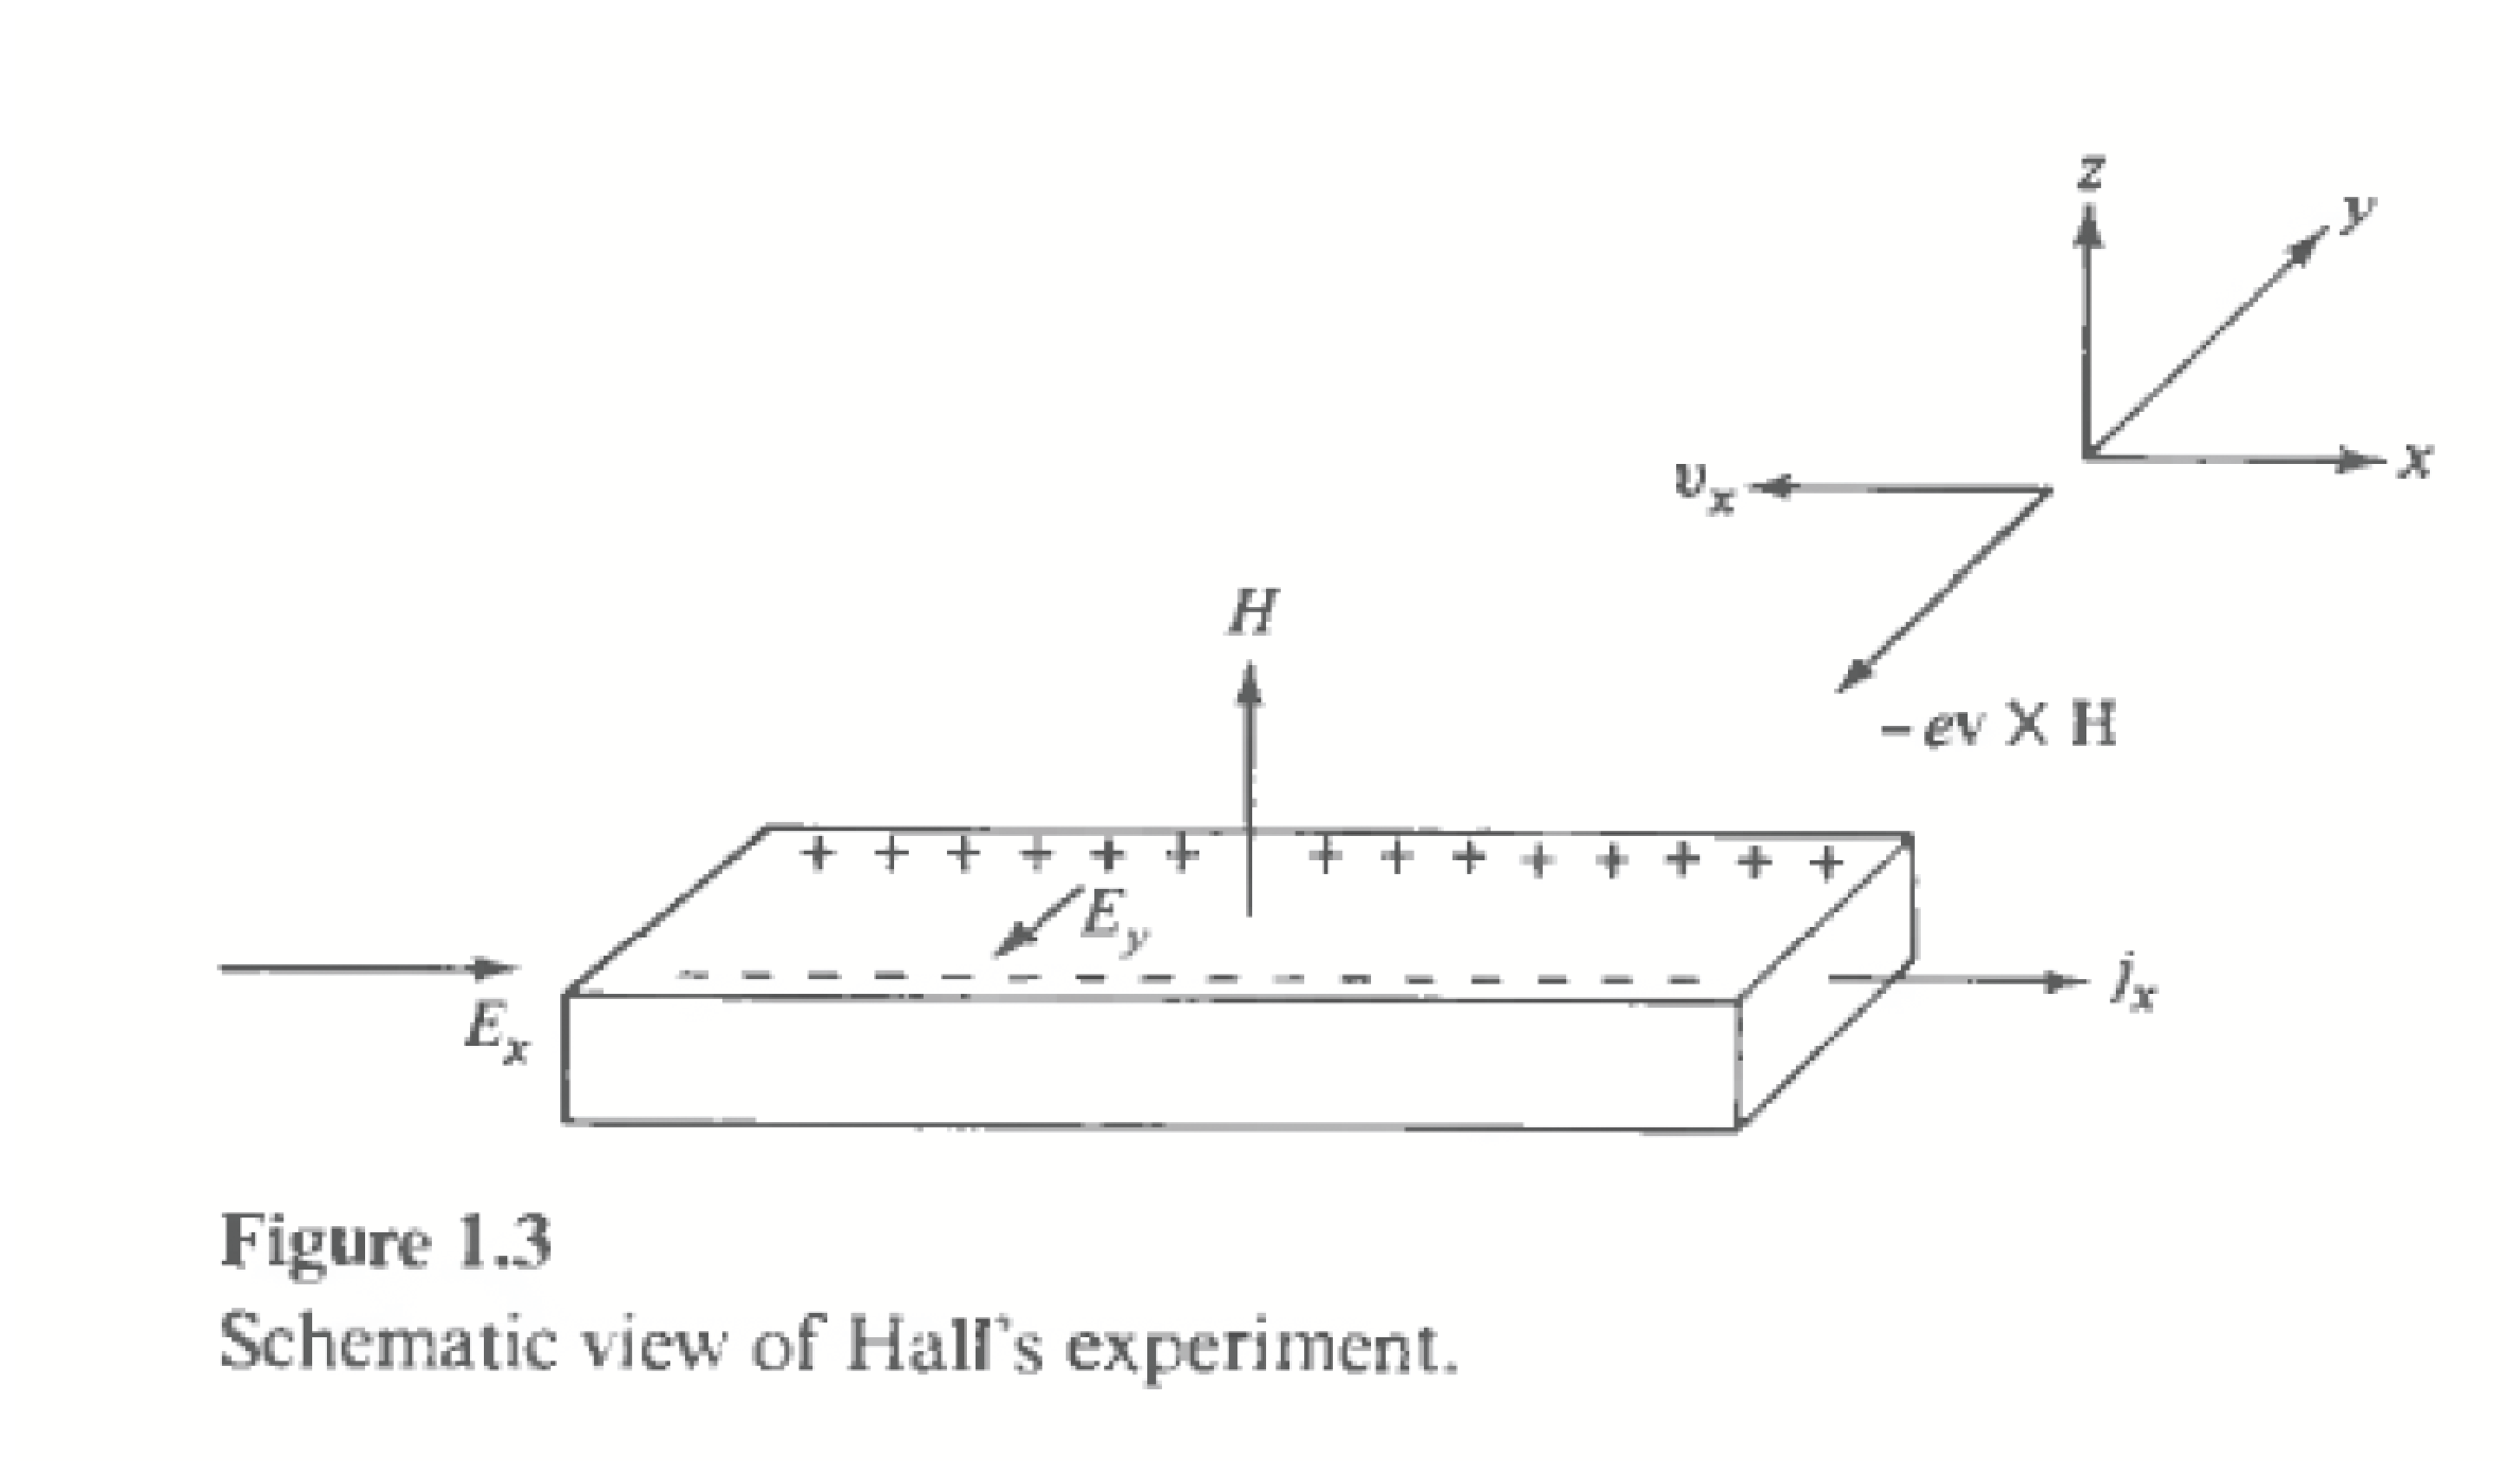
\includegraphics[width=0.7\textwidth]{CHE.eps}
\end{center}
\begin{block}
{Hall Effect}
\begin{itemize}
\item The Hall Effect is characterized by the induced potential that is perpendicular to both the current and the external magnetic field
\item The effect was first discovered by Edwin Hall in 1879
\end{itemize}
\end{block}
\end{frame}
\begin{frame}
\begin{block}
{Important results of the Hall Effect}
\begin{itemize}
\item The \emph{Hall Coefficient}, $R_H = -\dfrac{1}{nec}$, is independent of the of the properties of the substance except the density of the charge carriers, $n$ \cite{key1}.
\item The sign of $R_H$ determines the sign of the carriers charge.
\end{itemize}
\end{block}
\end{frame}

\begin{frame}
\frametitle{Landau Levels}
\begin{block}
{What is a Landau Level?}
\begin{itemize}
\item Landau Levels are quantized energy levels of charged particles in a cyclotron orbit due to an external magnetic field.
\item Landau levels are highly degenerate where the particles allowed per level is directly proportional to the applied magnetic field. 
\end{itemize}
\end{block}
\begin{block}
{Why do we care about Landau Levels?}
\begin{itemize}
\item The Quantum Hall Effect is directly related to Landau levels.
\item The Quantum Hall Effect occurs when you are in a two-dimensional system of charged particles in an external magnetic field.
\item Landau levels describe the energy levels of particles in this exact system.
\end{itemize}
\end{block}
\end{frame}

\begin{frame}
\begin{block}
{Brief Derivation of Landau Levels}
\begin{itemize}
\footnotesize{
\item We start with a simple system of non-interacting particles that only sit in a two-dimensional plane with an external magnetic field perpendicular to the plane.
\item This system is described by the Hamiltonian 
$$\hat{H} = \frac{1}{2m}\left(\hat{p} - \frac{q\hat{A}}{c}\right)^2$$
\item By using the \emph{gauge invariance} of the Hamiltonian and the fact that $\hat{P}_y$ commutes with $\hat{H}$ we can rewrite the Hamiltonian as
$$\hat{H} = \frac{\hat{p}_x^2}{2m} + \frac{1}{2}m\omega_c^2\left(\hat{x}-\frac{\hbar k_y}{m\omega_c}\right)^2$$
where the \emph{cyclotron frequency}, $\omega_c$, is defined as $\omega_c = Be/m$
\item The energy of this system is the same as the harmonic oscillator given as $E_n = \hbar\omega_c\left(n+\frac{1}{2}\right)$. The integer $n$ determines the Landau level. 
\item Note that each Landau level is highly degenerate. The number of states in filled level is given by $N_L = eB/h$ \cite{Klitz1980}
}
\end{itemize}
\end{block}
\end{frame}

\begin{frame}
\frametitle{Integer Quantum Hall Effect}
\begin{center}
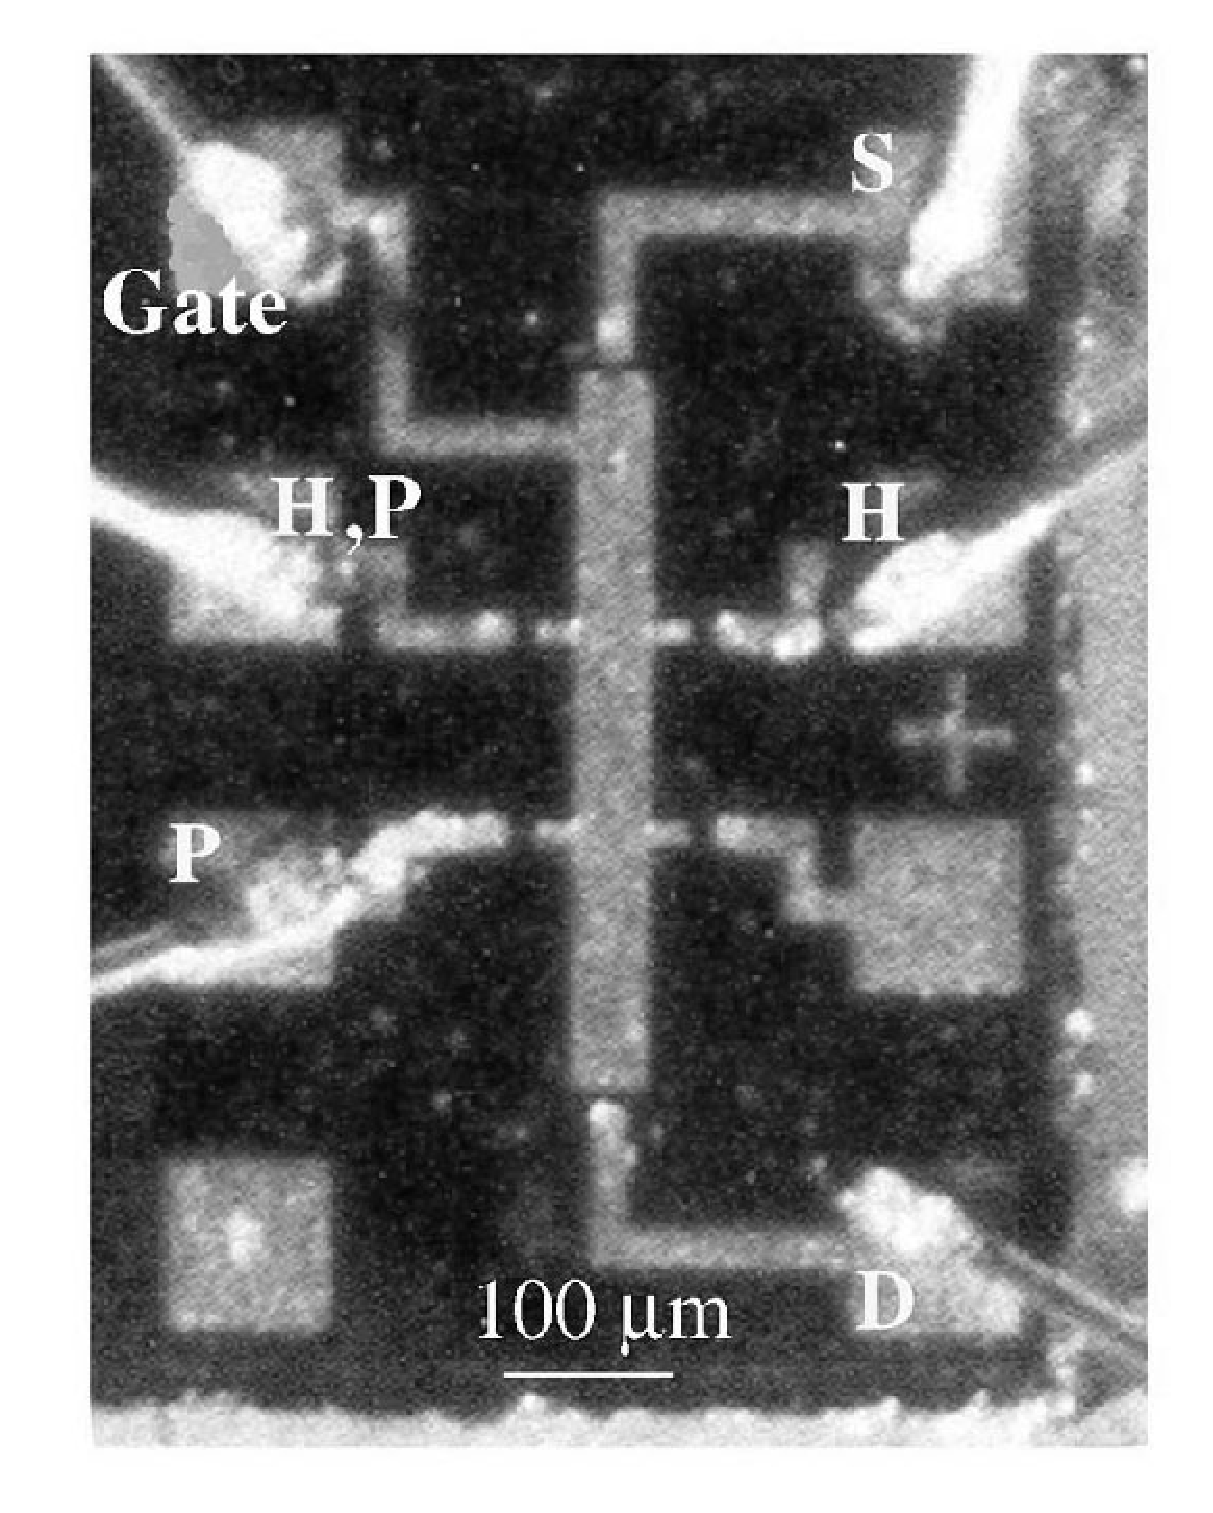
\includegraphics[scale=0.18]{QHEKlitz2.eps}
\end{center}
\begin{block}
{Discovery}
\begin{itemize}
\footnotesize{
\item The Integer Quantum Hall Effect was discovered by Klaus von Klitzing in 1980. He later won the Nobel Prize in 1985.
\item The experiment created a degenerate electron gas inside a MOSFET transistor. Then lowered the temperature of the transistor to $1.5$ K and placed it in a magnetic field of the order of $15$ T.
}
\end{itemize}
\end{block}
\end{frame}

\begin{frame}
\begin{center}
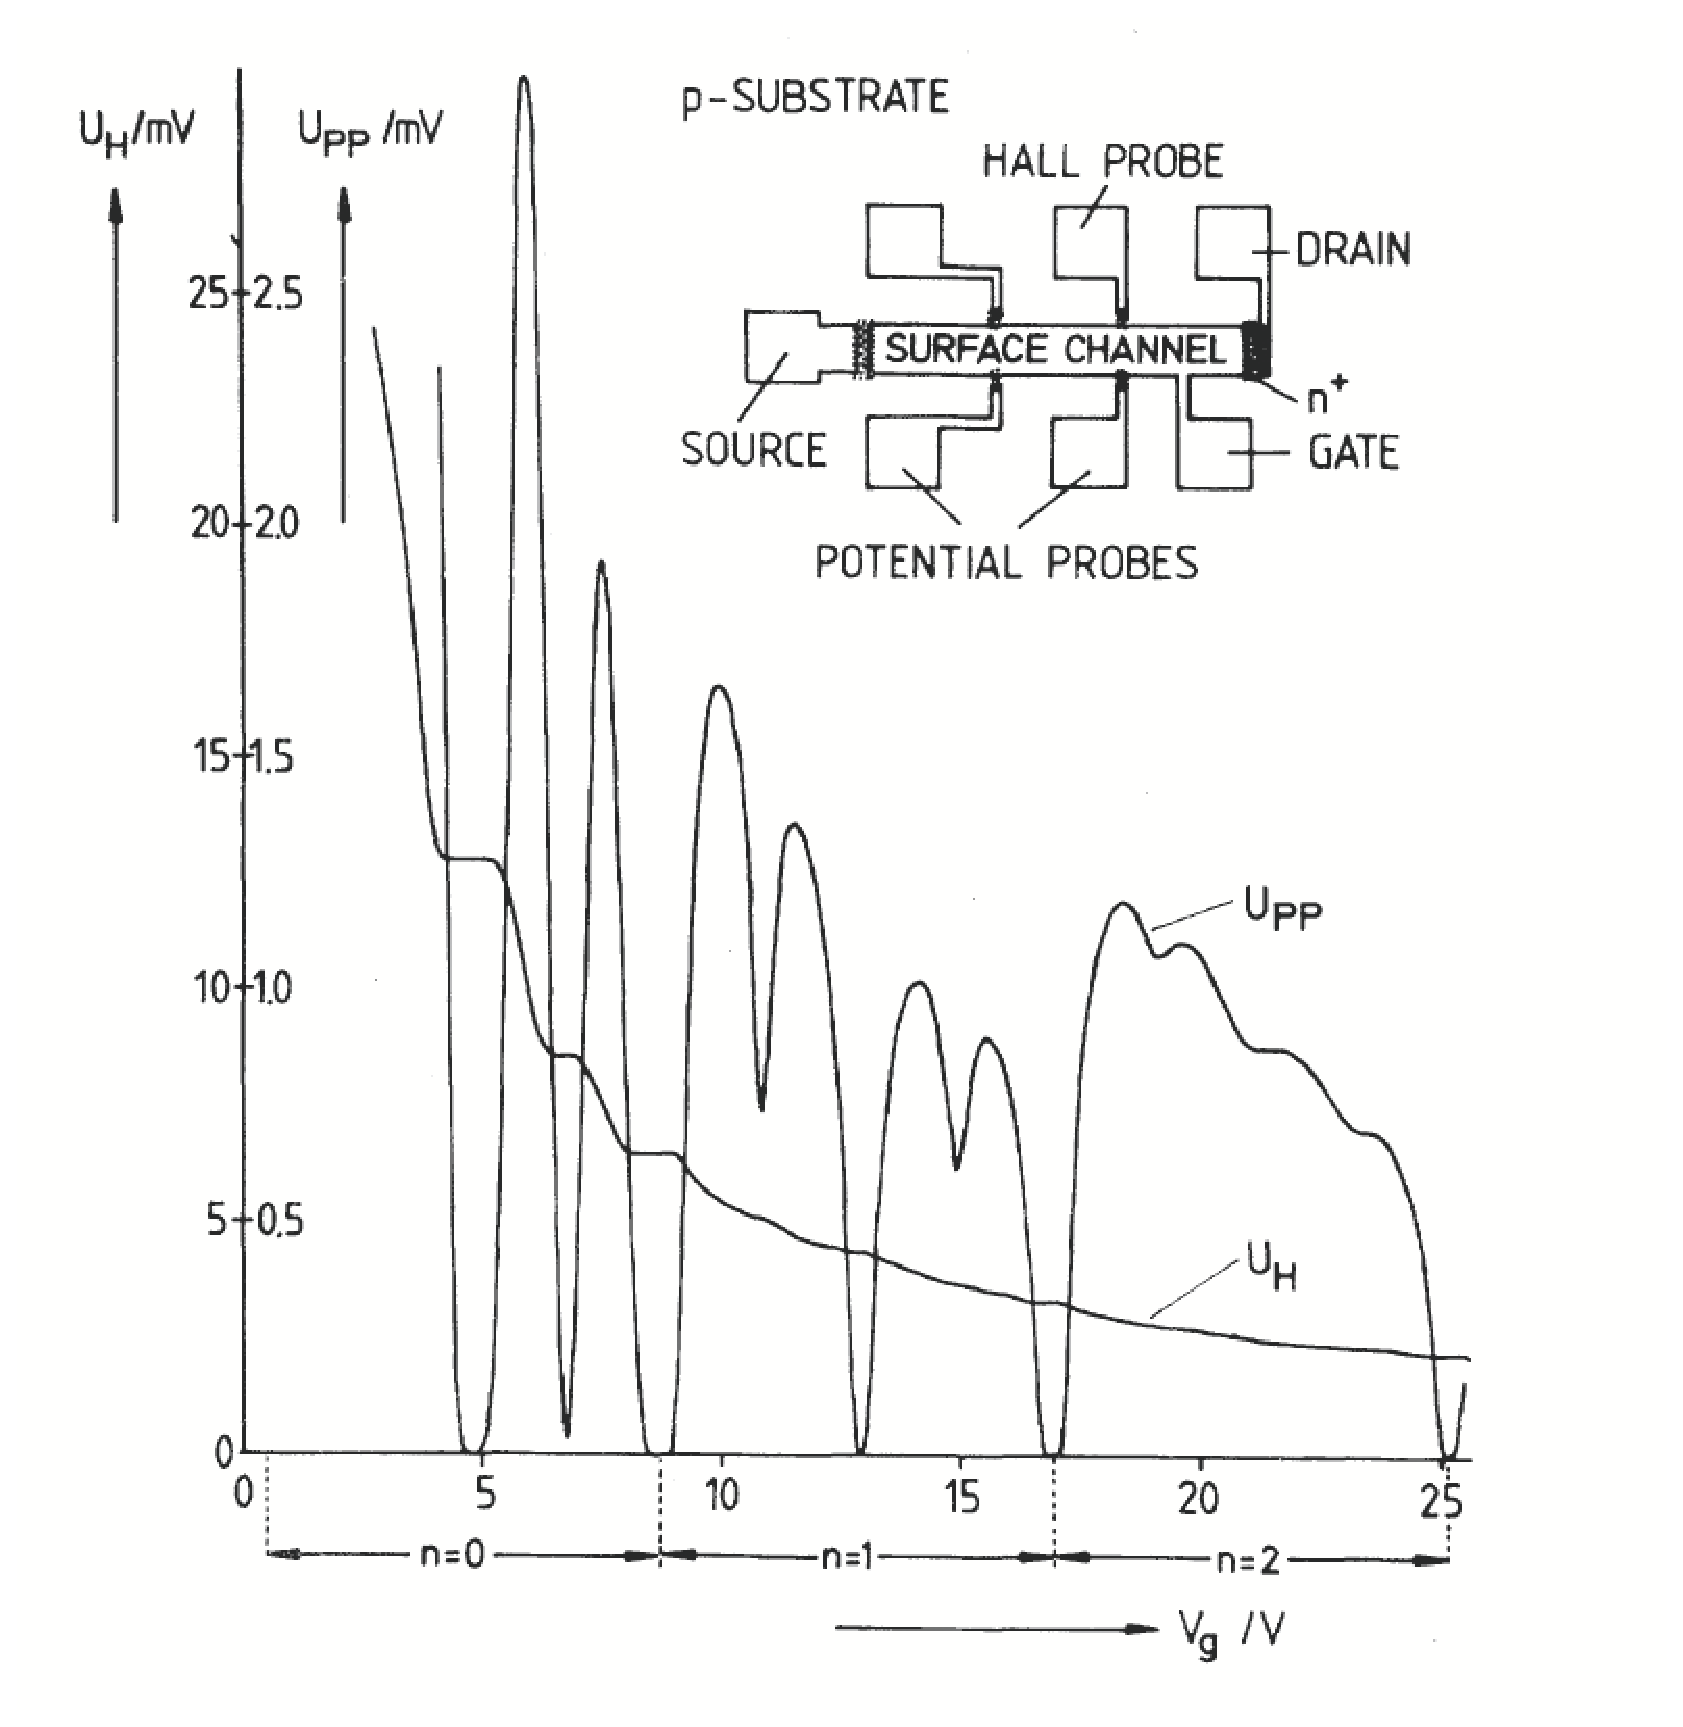
\includegraphics[width=0.4\textwidth]{QHEKlitz1.eps}
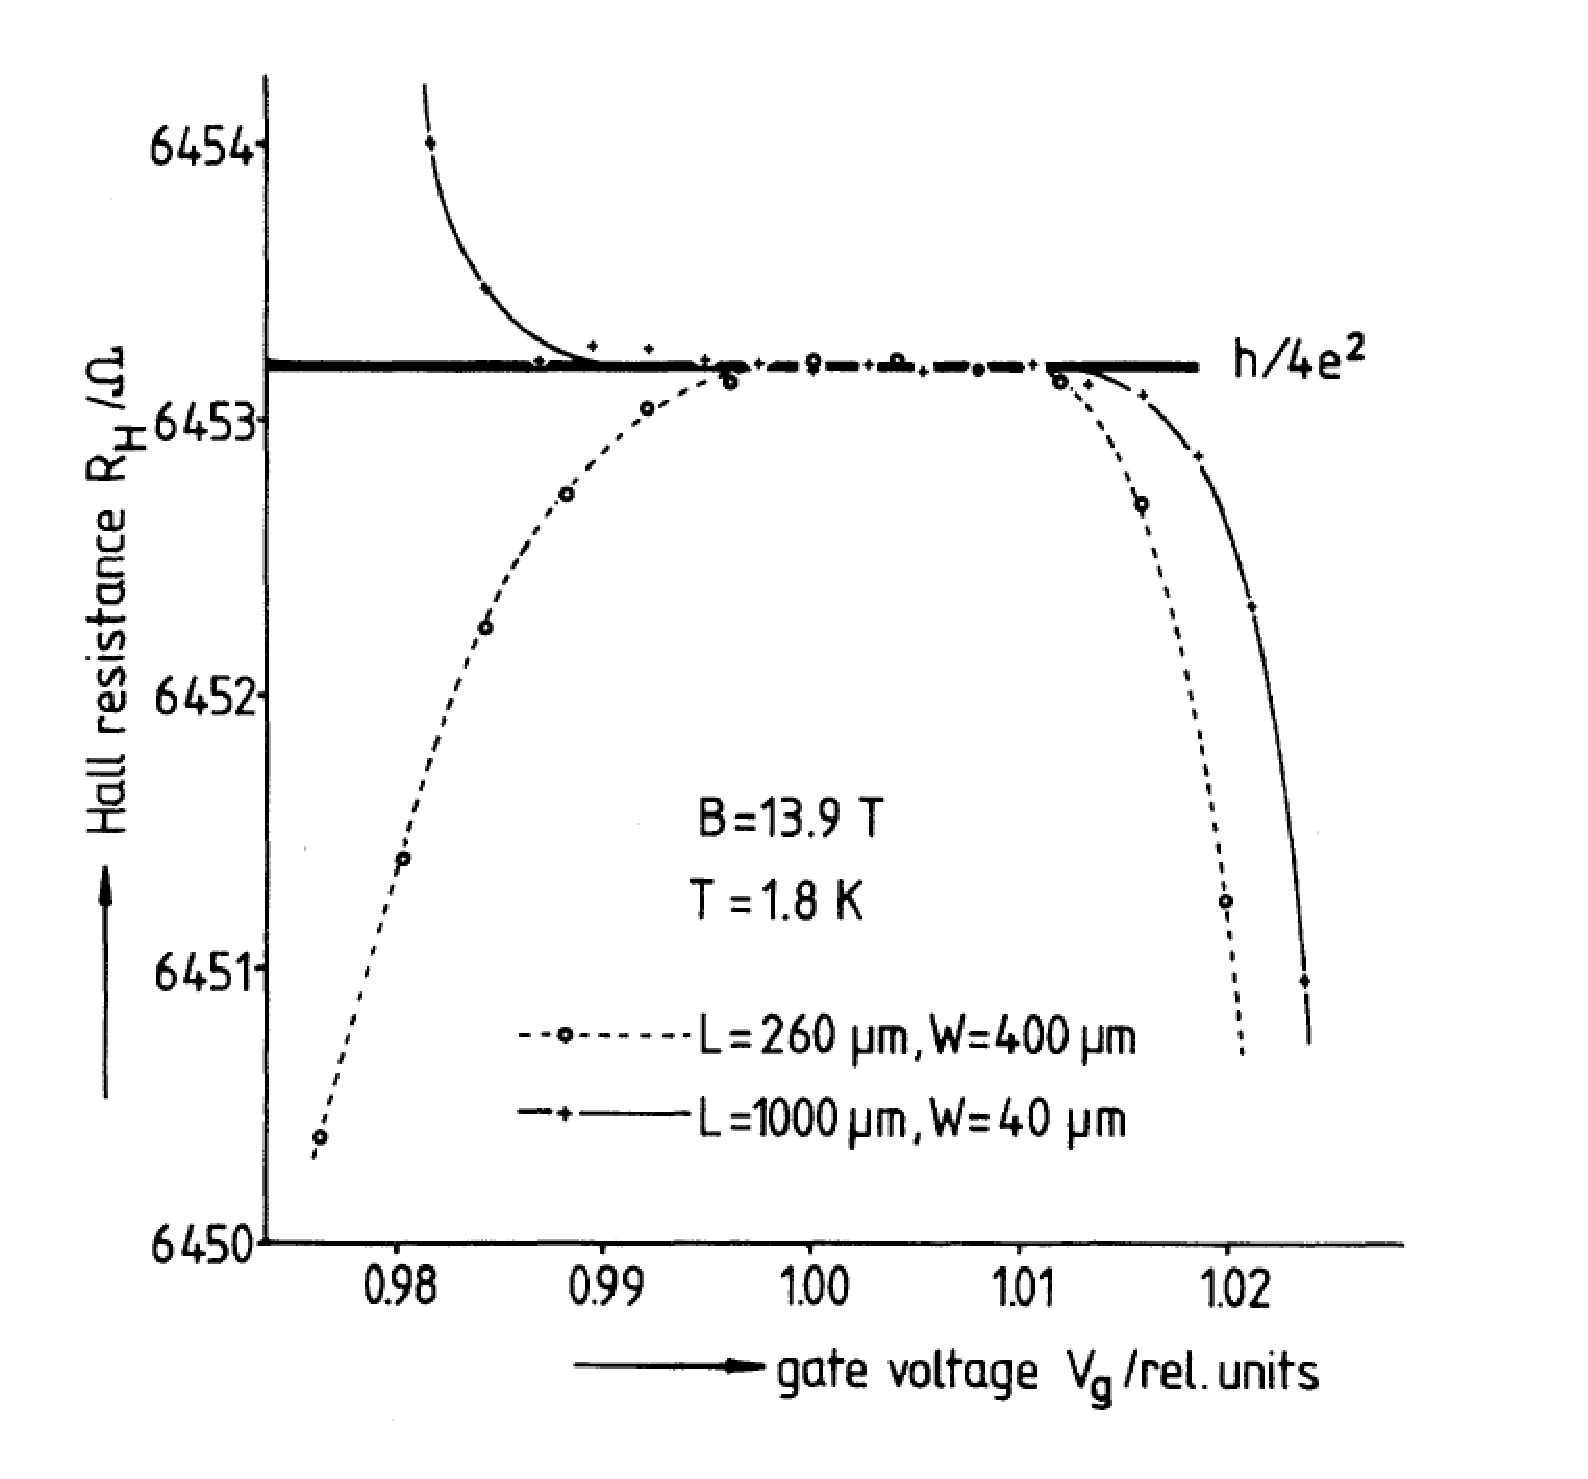
\includegraphics[width=0.4\textwidth]{QHEKlitz3.eps}
\end{center}
\begin{block}
{What did Klitzing find out?}
\begin{itemize}
\footnotesize{
\item Klitzing found that for a Fermi energy between Landau levels the Landau level is fully occupied with the number of states $N = N_Li$ where $i$ represents the Landau level and $i=1,2,3,...$. This lead to the quantization of the Hall conductivity by $-\sigma_{xy} = e^2i/h$.
\item He also found that the quantization was independent of the size and shape of the MOSFET. He then determined that the value was independent of geometry.
}
\end{itemize}
\end{block}
\end{frame}

\begin{frame}
\frametitle{Fractional Quantum Hall Effect}
\begin{columns}[T]
\begin{column}{0.5\textwidth}
\begin{center}
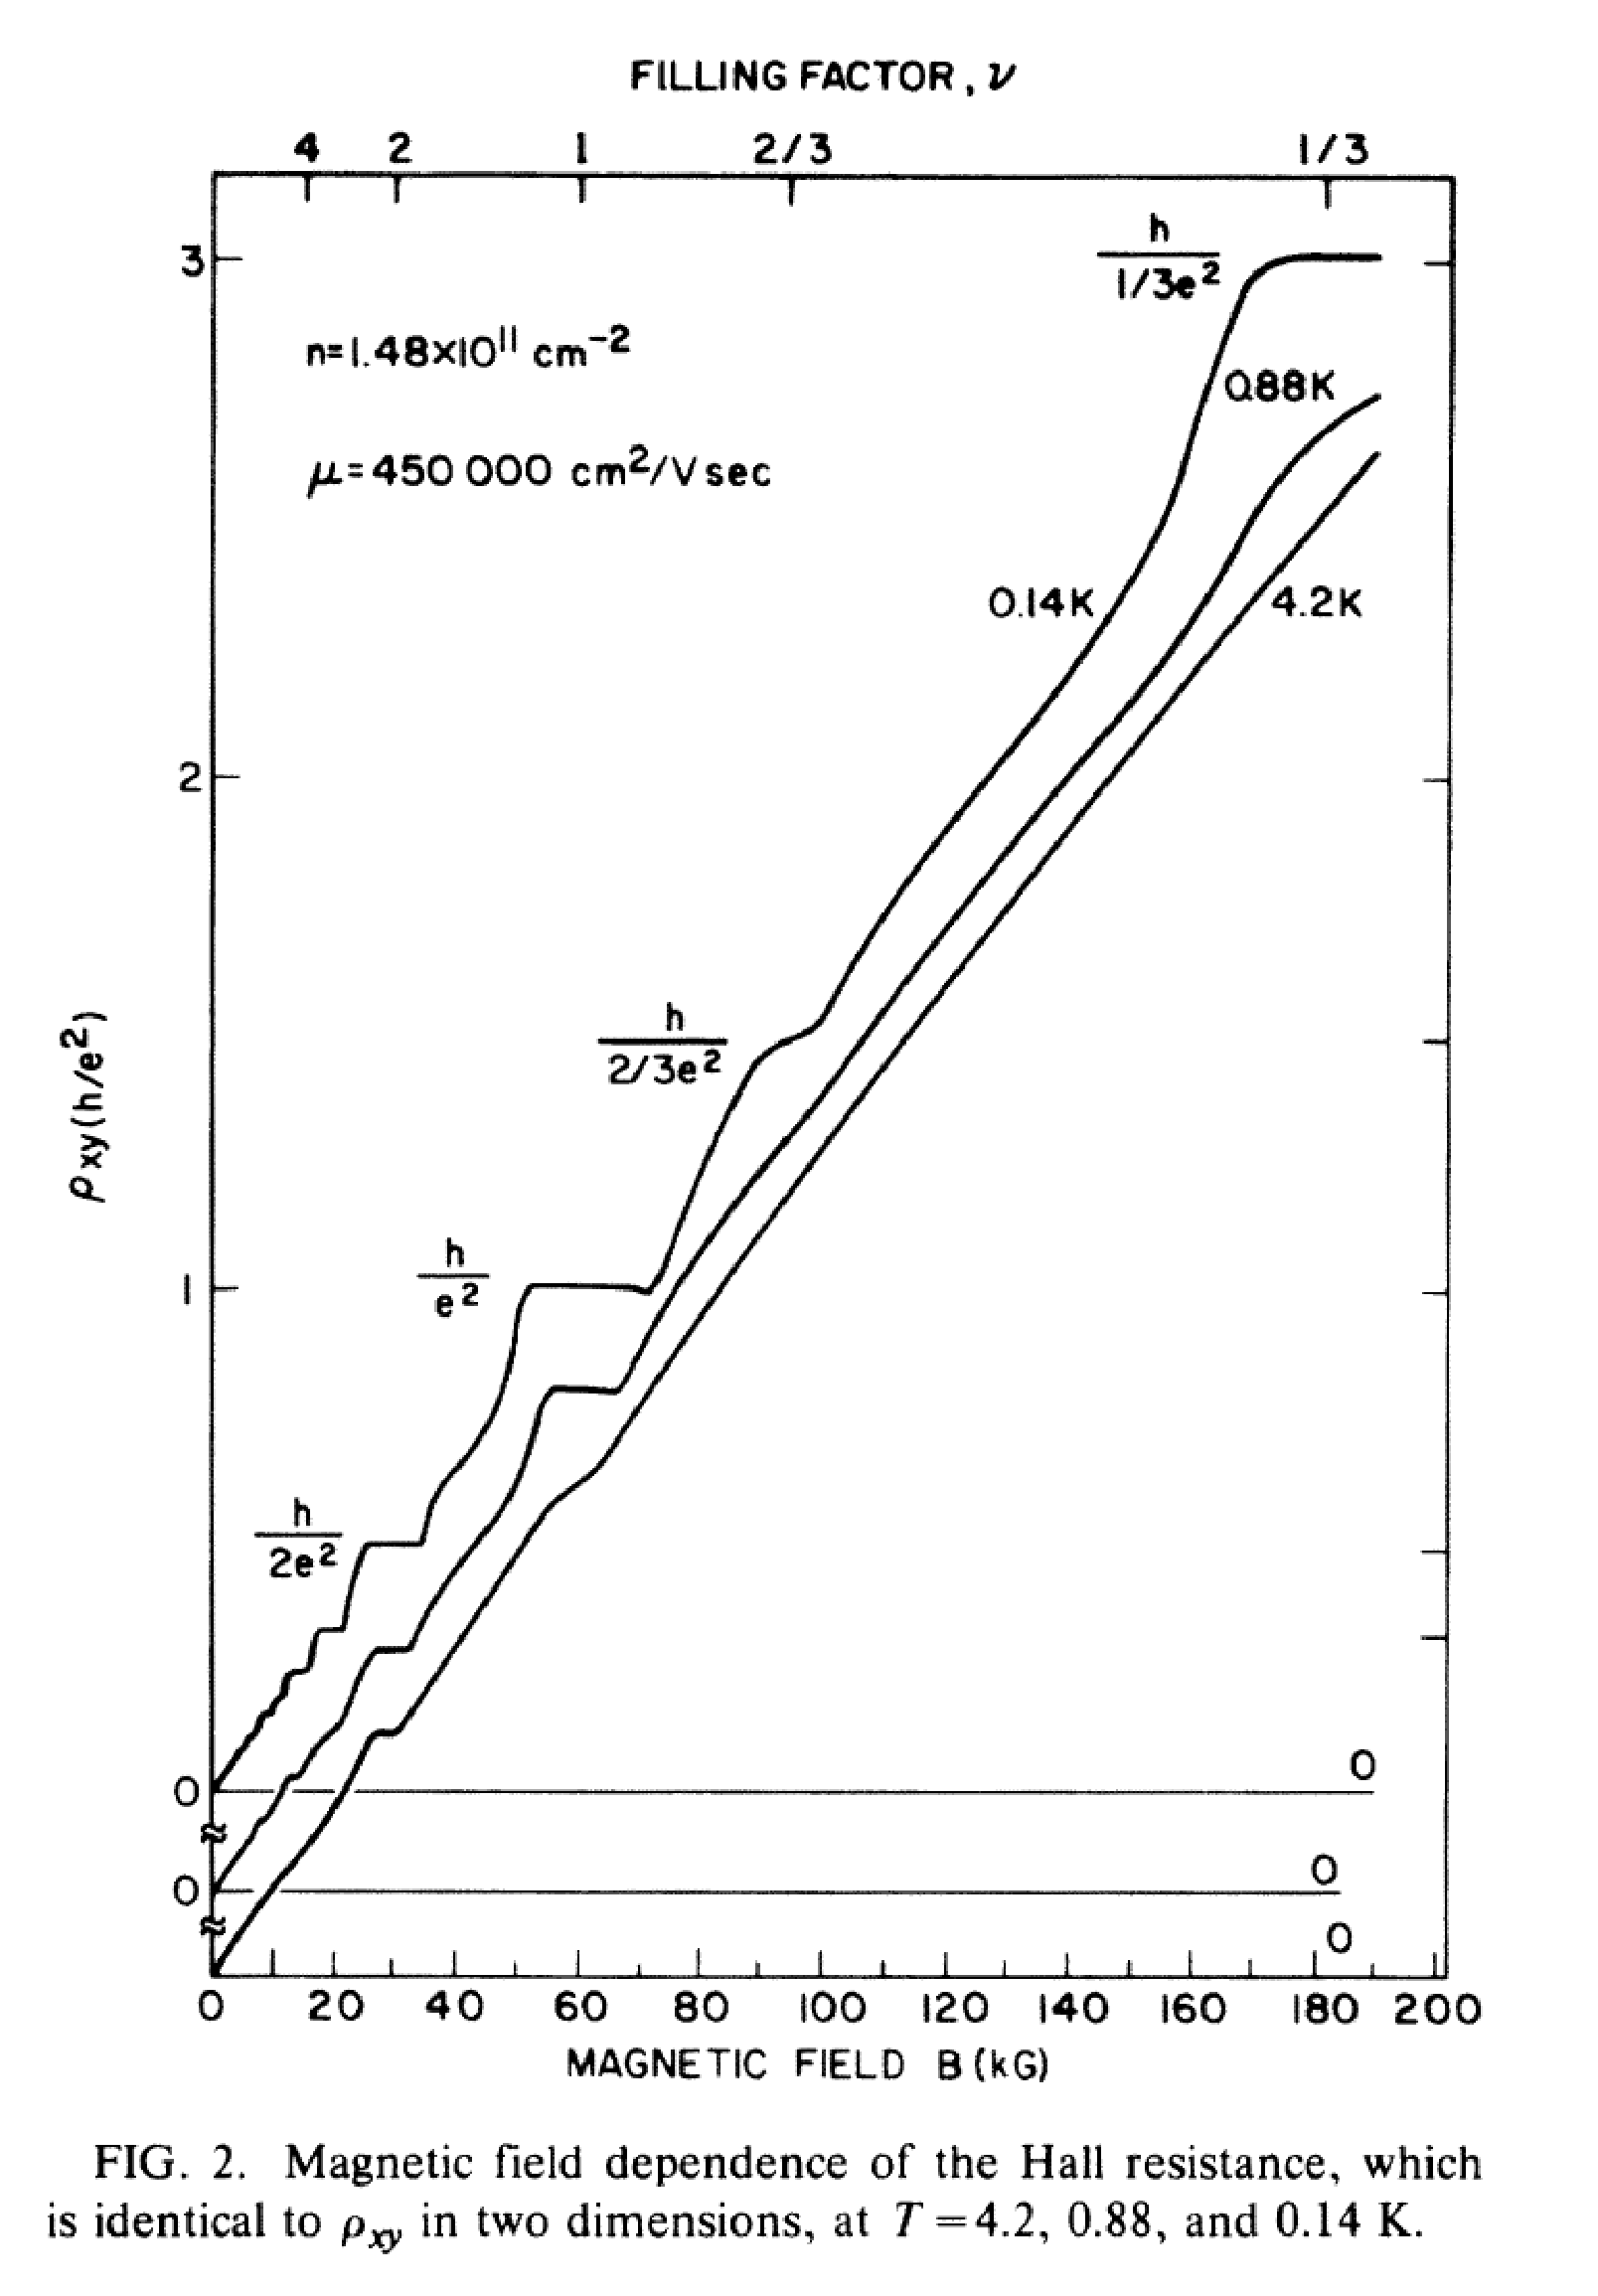
\includegraphics[width=0.9\textwidth]{Tsui1.eps}
\end{center}
\end{column}
\begin{column}{0.5\textwidth}
\begin{block}
{Discovery}
\begin{itemize}
\item By going to lower temperatures and newer semiconductors (to improve electron mobility) Daniel Tsui and Horst Stormer discovered a Landau level at 1/3 of a filled level in 1983. They later shared the Nobel Prize with Robert Laughlin in 1998
\item This result was not predicted by any theory at the time and was very unexpected.
\end{itemize}
\end{block}
\end{column}
\end{columns}
\end{frame}

\begin{frame}
\begin{block}
{Theoretical Description of the Fractional Quantum Hall Effect}
\begin{itemize}
\item In May of 1983 Robert Laughlin theorized that the Fractional Quantum Hall Effect was due to interactions between electrons. 
\item He predicted that in the limits where the Fractional Quantum Hall Effect was observed the electrons acted as an incompressible fluid.
\item He then drew an analogy to charged particles in a plasma and that in the plasma charge would get shielded by other moving charges.
\item This lead Laughlin to conclude that the electrons and holes acted like quasielectrons and quasiholes. Which are virtual particles with fractional charge.
\end{itemize}
\end{block}
\end{frame}
 
\begin{frame}
\frametitle{Citations}
\footnotesize{
\begin{thebibliography}{99}
 \bibitem[1]{key1} N. W. Ashcroft and N. D. Mermin, \emph{Solid State Physics} (Holt Rinehart and Winston, New York ,1976), pp. 11-15.
 \bibitem[2]{Klitz1980} K. Klitzing, \emph{Phys. Rev. Lett.} \textbf{45,} 494 (1980)
 \bibitem[3]{TsuiAug1983} D. C. Tsui et al, \emph{Phys. Rev. B} \textbf{28,} 2274 (1983)
 \bibitem[4]{Klitz2005} K. Klitzing, http://hrma.physics.sjtu.edu.cn/PhysicsHorizon/25yearsQHE-lecture.pdf
 \bibitem[5]{Ando1975}T. Ando, Y Matsumoto, and Y. Uemura, \emph{J. Phys. Soc. Jpn.} \textbf{39,} (1975) pp. 279-288
 \bibitem[6]{Laug1981}R. B. Laughlin \emph{Phys. Rev. B} \textbf{23,} 5632 (1981)
 \bibitem[7]{TsuiMay1982}D. C. Tsui, H. L. Stormer, and A. C. Gossard, \emph{Phys. Rev. Lett.} \textbf{48,} 1559 (1982)
 \bibitem[8]{Laug1983}R. B. Laughlin \emph{Phys. Rev. Lett.} \textbf{50,} 1395 (1983)
\end{thebibliography}
}
\end{frame}
 
% End of slides
\end{document} 

